%%----------------------------------------------------------
%% report_temp.tex
%% v1.0
%% 2022/10/28
%% by Carlos Rodríguez - Pardo, 2023, Universidad Carlos III de Madrid
%%----------------------------------------------------------

\documentclass{wsdcr}
\usepackage[spanish]{babel}
\usepackage{booktabs}
\usepackage{multirow}
\usepackage{markdown}
\usepackage{graphicx}


\title{%
    Predictor de bicicletas prestadas \\
    \large Análisis Avanzado de Datos - Práctica Final }
\author{Alejo Martín, Arias Filippo (NIA: 100487858)}
\date{2023}

\begin{document}

\maketitle

\section{Introducción}
Los sistemas de bicicletas compartidas se han vuelto muy populares en todo el mundo debido a su capacidad para mejorar la movilidad urbana, la salud y el medio ambiente. Estos sistemas generan grandes cantidades de datos que pueden ayudarnos a comprender mejor cómo se mueven las personas en las ciudades y qué eventos importantes ocurren en ellas. En este proyecto, vamos a utilizar un conjunto de datos de un sistema de bicicletas compartidas para construir un modelo de aprendizaje supervisado que prediga la cantidad de bicicletas alquiladas en función de diferentes factores, como la hora del día, la temperatura, la humedad y las condiciones meteorológicas.

El objetivo principal de este proyecto es mostrar cómo el aprendizaje supervisado puede ser útil para predecir la demanda de bicicletas compartidas según las condiciones ambientales y temporales, lo que podría ayudar a los operadores del sistema a mejorar la disponibilidad de bicicletas y a satisfacer mejor las necesidades de los clientes. Para lograr este objetivo, vamos a seguir un enfoque de aprendizaje supervisado, utilizando un conjunto de datos etiquetados para entrenar un modelo que pueda predecir la cantidad de bicicletas alquiladas según los diferentes factores que hemos mencionado.


\section{Descripción del Dataset}
El dataset utilizado en este proyecto es un conjunto de registros de préstamos de bicicletas compartidas en un sistema automatizado. Contiene información sobre más de 17,000 préstamos realizados cada hora durante un período de dos años, desde enero de 2011 hasta diciembre de 2012. Cada registro contiene detalles importantes, como la fecha y hora del préstamo, las condiciones climáticas, y la cantidad de bicicletas alquiladas por usuarios registrados y ocasionales.

El dataset consta de 15 columnas que proporcionan información útil sobre los patrones de préstamo de bicicletas. Las primeras columnas incluyen detalles sobre el día y la hora del préstamo, así como la temporada, el año, el mes, el día de la semana y si es un día laborable o festivo. También se registran la temperatura, la sensación térmica, la humedad y la velocidad del viento. Además, la columna "weathersit" indica las condiciones climáticas generales en la hora del préstamo. Finalmente, se incluyen tres columnas que registran el número de bicicletas alquiladas por usuarios ocasionales, usuarios registrados y el número total de bicicletas alquiladas.

\begin{itemize}
    \item \textbf{Instant}: Este es el índice de registro y no tiene un valor informativo por sí mismo.
    \item \textbf{Dteday}: Esta variable indica la fecha en que se realizó el préstamo. La fecha está en formato año-mes-día.
    \item \textbf{Hr}: Esta variable indica la hora del día en que se realizó el préstamo.
    \item \textbf{Season}: Esta variable indica la temporada en la que se realizó el préstamo. Los valores son 1 (primavera), 2 (verano), 3 (otoño) y 4 (invierno).
    \item \textbf{Year}: Esta variable indica el año en que se realizó el préstamo.
    \item \textbf{Mnth}: Esta variable indica el mes en que se realizó el préstamo.
    \item \textbf{Holiday}: Esta variable indica si el día en que se realizó el préstamo era un día festivo (1) o no (0).
    \item \textbf{Weekday}: Esta variable indica el día de la semana en que se realizó el préstamo. Los valores son 0 (domingo) a 6 (sábado).
    \item \textbf{Workingday}: Esta variable indica si el día en que se realizó el préstamo era un día laborable (1) o no (0).
    \item \textbf{Weathersit}: Esta variable indica las condiciones climáticas generales en la hora del préstamo. Los valores son 1 (despejado), 2 (nublado), 3 (lluvia ligera/nieve ligera) y 4 (lluvia intensa/nieve intensa).
    \item \textbf{Temp}: Esta variable indica la temperatura en grados Celsius en el momento del préstamo.
    \item \textbf{Atemp}: Esta variable indica la sensación térmica en grados Celsius en el momento del préstamo.
    \item \textbf{Hum}: Esta variable indica la humedad relativa en el momento del préstamo.
    \item \textbf{Windspeed}: Esta variable indica la velocidad del viento en km/h en el momento del préstamo.
    \item \textbf{Casual}: Esta variable indica el número de bicicletas alquiladas por usuarios ocasionales en la hora del préstamo.
    \item \textbf{Registered}: Esta variable indica el número de bicicletas alquiladas por usuarios registrados en la hora del préstamo.
    \item \textbf{Count}: Esta variable indica el número total de bicicletas alquiladas en la hora del préstamo (es decir, la suma de los valores de las variables Casual y Registered).
\end{itemize}

\section{Descripción del problema}
En este proyecto, nuestro objetivo es predecir el número de bicicletas que se alquilarán en una hora determinada utilizando un modelo de aprendizaje supervisado. Para lograr esto, vamos a considerar varias variables que podrían influir en la cantidad de bicicletas alquiladas.

Una de las variables más importantes es la hora del día, ya que se espera que la cantidad de bicicletas alquiladas varíe a lo largo del día debido a los patrones de movilidad de las personas. Es posible que haya más alquileres de bicicletas durante las horas pico de la mañana y la tarde, cuando la gente se dirige al trabajo o regresa a casa.

Otra variable importante es el clima. Las condiciones climáticas pueden tener un gran impacto en la cantidad de bicicletas alquiladas. Es posible que haya menos alquileres de bicicletas en días lluviosos o fríos, mientras que en días soleados y cálidos se pueden alquilar más bicicletas.

Además, las variables de temperatura, humedad y velocidad del viento también pueden tener un efecto en la cantidad de bicicletas alquiladas. Es posible que las personas estén menos dispuestas a alquilar bicicletas en días extremadamente calurosos o húmedos.

Finalmente, es importante tener en cuenta las variables relacionadas con los usuarios, como la cantidad de usuarios registrados y ocasionales. Es posible que los patrones de alquiler difieran según el tipo de usuario y que los usuarios registrados alquilen bicicletas con más frecuencia que los usuarios ocasionales.

\section{Análisis de los datos}

\begin{verbatim}
    |            |       cnt |
    |:-----------|----------:|
    | instant    |  0.278379 |
    | weekday    |  0.0268999|
    | workingday |  0.0302844|
    | weathersit | -0.142426 |
    | atemp      |  0.400929 |
    | windspeed  |  0.0932338|
    | hum        | -0.322911 |
    | casual     |  0.694564 |
    | registered |  0.972151 |
    | cnt        |  1        |
\end{verbatim}

La tabla muestra la correlación entre la variable dependiente \textit{cnt} (número total de bicicletas alquiladas) y las diferentes variables independientes en el conjunto de datos.

Se puede observar que la variable más fuertemente correlacionada con \textit{cnt} es \textit{registered} (correlación positiva de 0.972), que representa el número de usuarios registrados que alquilan bicicletas. La variable \textit{casual} (correlación positiva de 0.695) también tiene una fuerte correlación con \textit{cnt}, lo que indica que los usuarios no registrados también tienen un impacto significativo en el número total de bicicletas alquiladas.

Además, se puede observar una correlación positiva moderada entre \textit{cnt} y \textit{atemp} (0.401), que representa la temperatura ajustada. Esto sugiere que los usuarios tienen más probabilidades de alquilar bicicletas en días con temperaturas más cálidas.

Por otro lado, se puede observar una correlación negativa moderada entre \textit{cnt} y \textit{hum} (-0.323), que representa la humedad. Esto sugiere que los usuarios tienen menos probabilidades de alquilar bicicletas en días más húmedos.

Finalmente, \textit{weathersit} (condiciones meteorológicas) y \textit{windspeed} (velocidad del viento) tienen una correlación débil y negativa con \textit{cnt}, lo que sugiere que estos factores no tienen un impacto significativo en el número total de bicicletas alquiladas.


\begin{figure}[h]
    \centering
    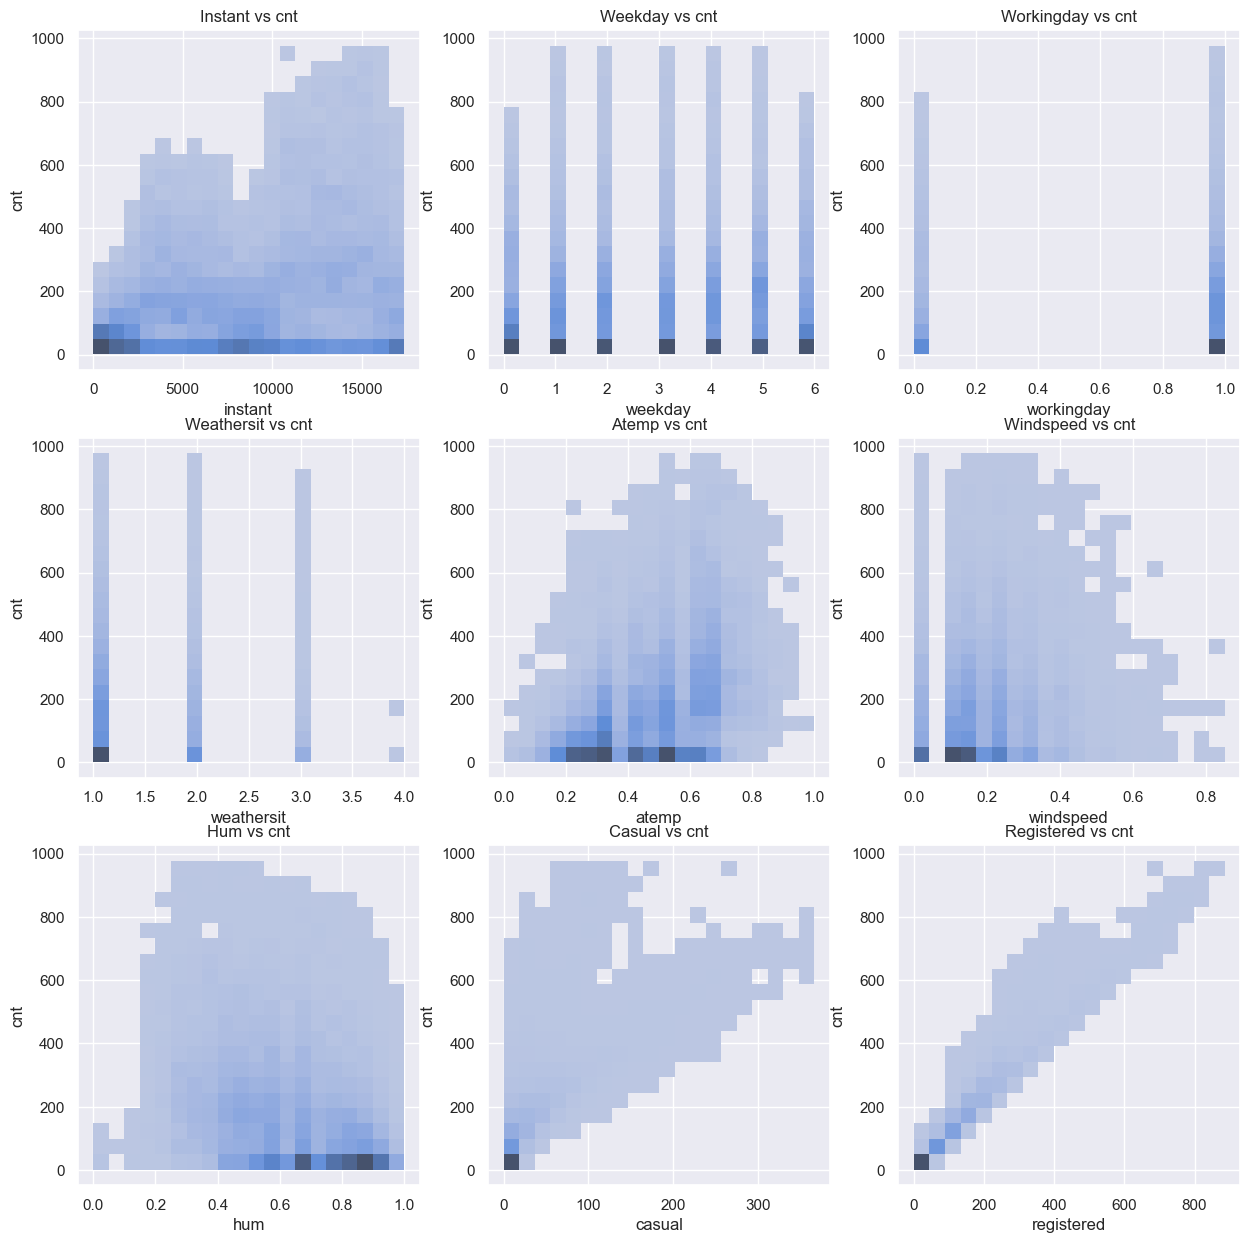
\includegraphics[width=0.4\textwidth]{charts/histograms.png}
    \caption{Histogramas}
    \label{fig:histograms}
\end{figure}

\begin{figure}[h]
    \centering
    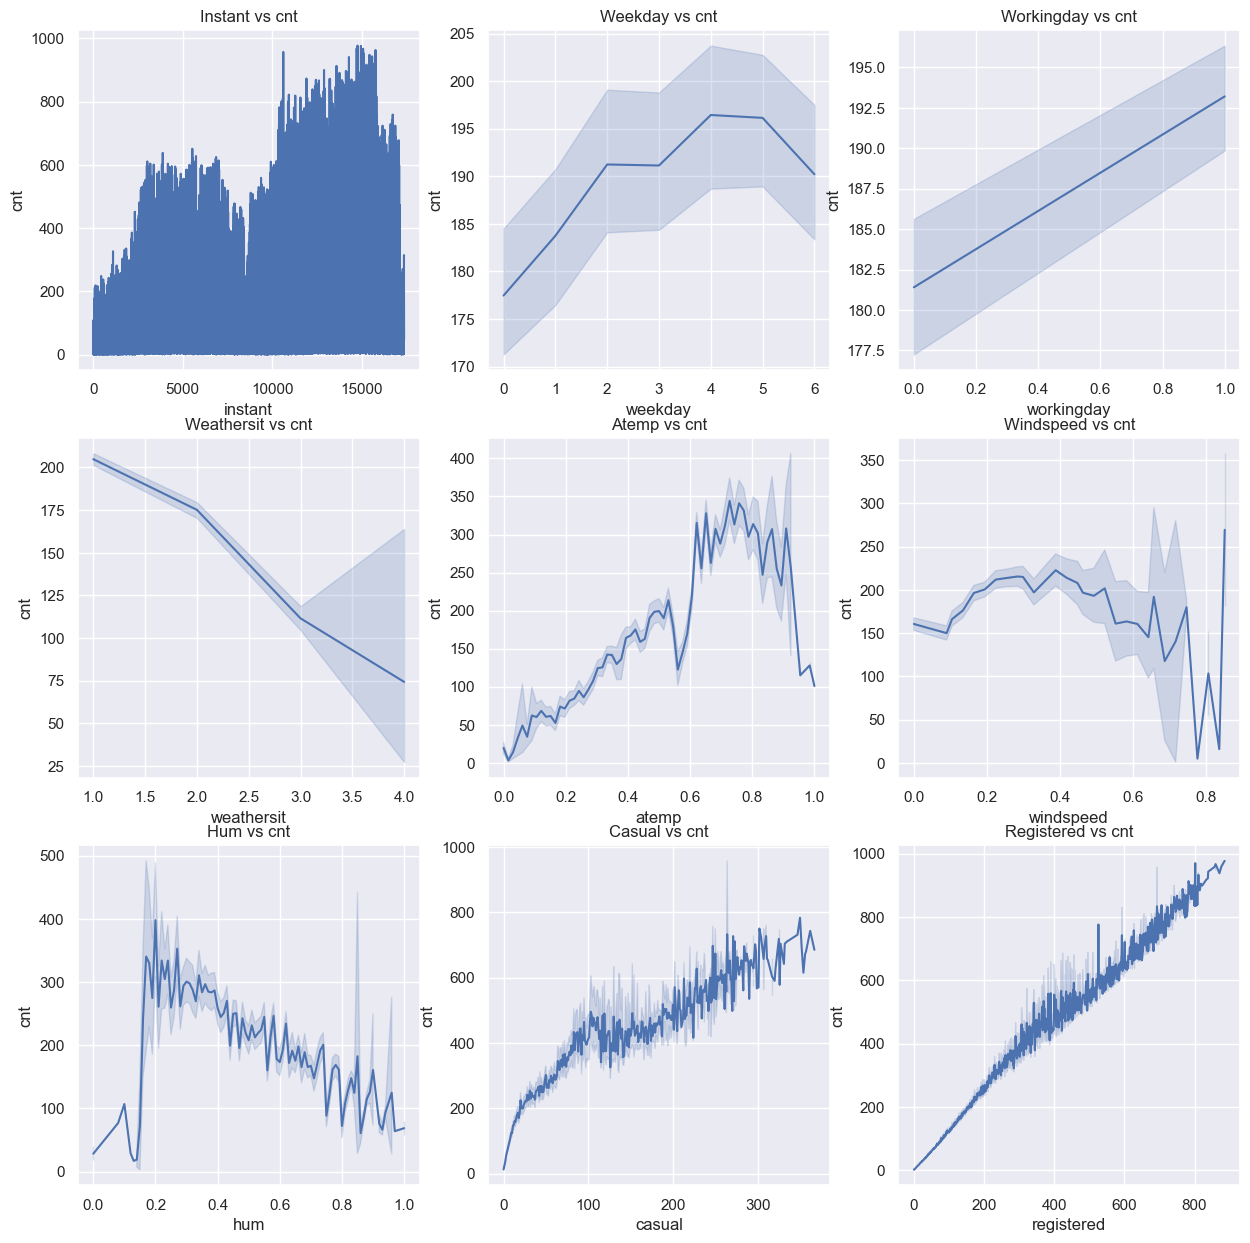
\includegraphics[width=0.4\textwidth]{charts/line-charts.png}
    \caption{Gráfico de líneas}
    \label{fig:linecharts}
\end{figure}

\begin{figure}[h]
    \centering
    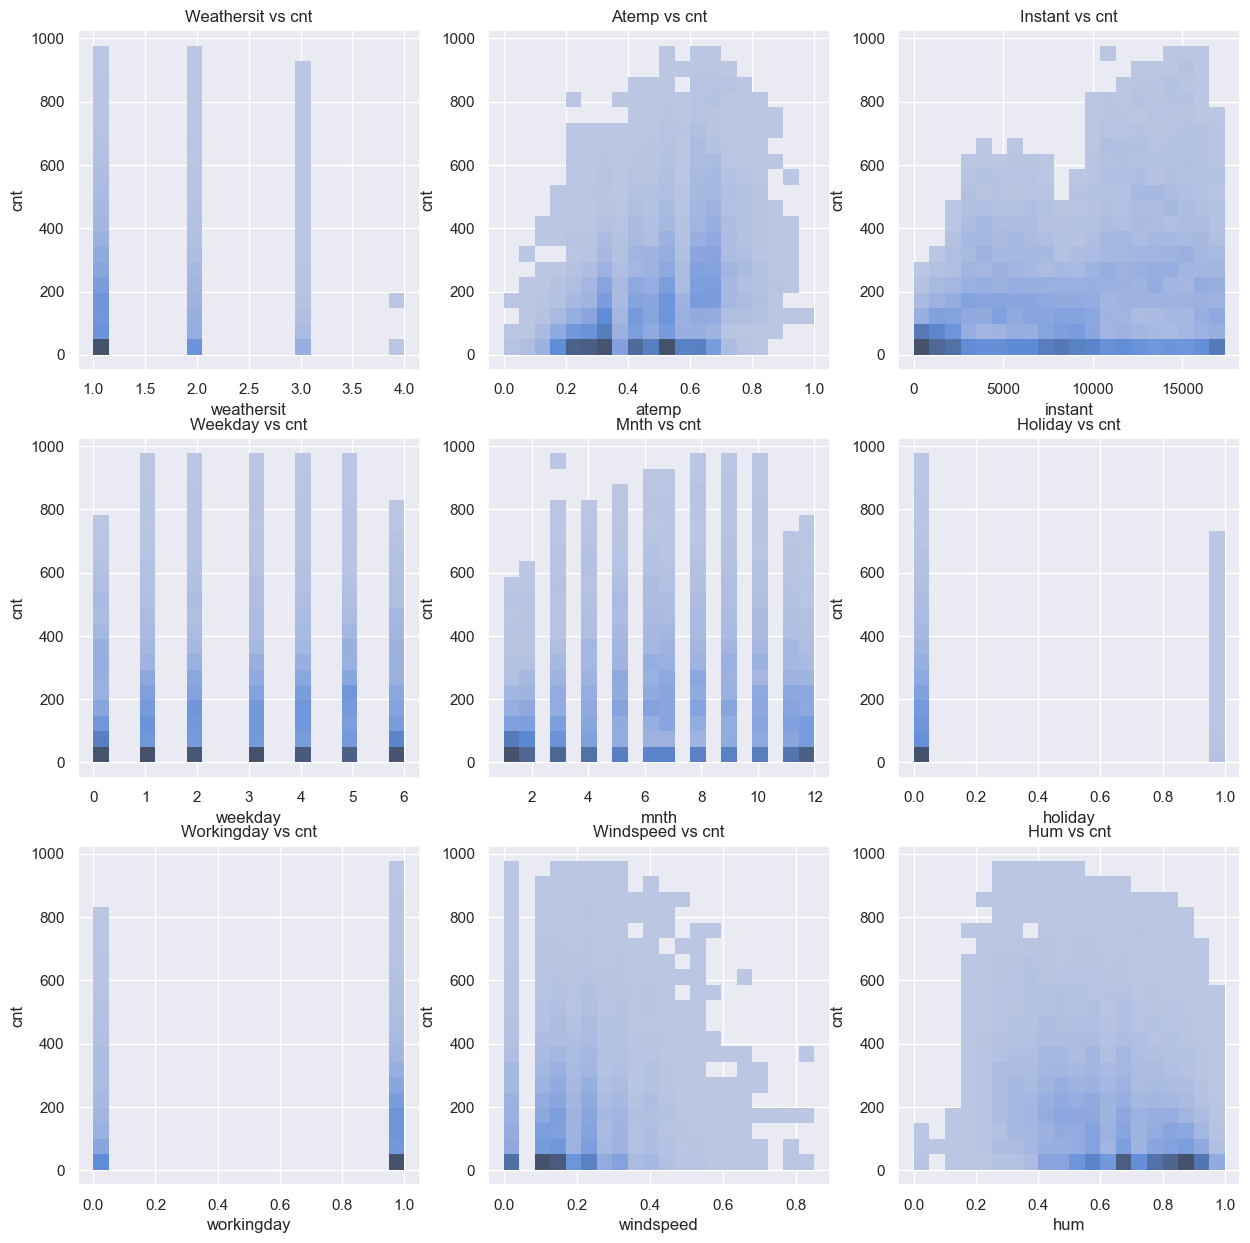
\includegraphics[width=0.4\textwidth]{charts/correlational-matrix.png}
    \caption{Matriz correlacional}
    \label{fig:correlationmatrix}
\end{figure}

Para obtener los histogramas, utilizamos la función hist de la librería matplotlib, que nos permite visualizar la distribución de cada variable. Para obtener los gráficos de líneas correlacional, utilizamos la función plot de la misma librería, pasando como parámetros las variables a graficar y la variable cnt. Finalmente, para obtener la matriz correlacional, utilizamos la función heatmap de la librería seaborn.

Estos gráficos nos permiten visualizar las relaciones entre las variables y la variable cnt. Los histogramas nos muestran la distribución de cada variable, mientras que los gráficos de líneas correlacional nos permiten ver la relación entre cada variable y cnt. La matriz correlacional nos muestra la relación entre todas las variables.

De esta forma, podemos relacionar las conclusiones obtenidas en la última tabla con los gráficos obtenidos. Por ejemplo, la correlación positiva entre la variable atemp y cnt se refleja en el gráfico de líneas correlacional correspondiente, donde podemos ver una tendencia positiva entre ambas variables. Del mismo modo, la correlación negativa entre hum y cnt se refleja en el gráfico correspondiente, donde podemos ver una tendencia negativa entre ambas variables. Los histogramas nos muestran la distribución de cada variable y nos permiten ver si hay valores atípicos o si los datos siguen una distribución normal. La matriz correlacional nos muestra todas las correlaciones entre las variables, lo que nos permite tener una visión general de la relación entre todas las variables en conjunto.

\section{Método}

\subsection{Aprendizaje supervisado}
En primer lugar, dividiremos nuestros datos en un conjunto de entrenamiento y un conjunto de prueba. A continuación, aplicaremos diferentes técnicas de regresión, como la regresión lineal o la regresión polinómica, para modelar la relación entre las variables independientes (día de la semana, hora del día, temperatura, etc.) y la variable dependiente (número de bicicletas alquiladas).

Una vez que hayamos entrenado nuestro modelo de regresión, evaluaremos su rendimiento utilizando diferentes métricas, como el error cuadrático medio o el coeficiente de determinación. Si nuestro modelo tiene un buen rendimiento en el conjunto de prueba, lo utilizaremos para hacer predicciones sobre la demanda futura de bicicletas.

\subsection{Aprendizaje no supervisado}
Se utilizaran ténicas de clustering y reducción de dimensionalidad.
En el caso del clustering, agruparíamos los datos en diferentes grupos o clústeres según su similitud, lo que nos permitiría identificar patrones y características comunes en los datos. Esto podría ser útil para segmentar la demanda de bicicletas y detectar posibles oportunidades de negocio.

Por otro lado, la reducción de dimensionalidad nos permitiría reducir el número de variables o características en nuestros datos sin perder información importante. Esto podría ser útil si tenemos un gran número de variables y queremos simplificar nuestro modelo de regresión sin perder precisión en nuestras predicciones.
\subsubsection{Etiquetado de los datos y su importancia en el aprendizaje no supervisado}

El etiquetado de los datos es una técnica importante en el aprendizaje no supervisado que nos permite asignar categorías o etiquetas a los datos en función de ciertos criterios. Al asignar etiquetas a los datos, podemos transformar un conjunto de datos no etiquetado en uno etiquetado que puede ser utilizado para evaluar el rendimiento de un modelo de aprendizaje no supervisado. También puede ayudar a identificar patrones y relaciones subyacentes en los datos que no serían evidentes de otra manera.

En este caso, el etiquetado se realizó en función del valor total de bicicletas alquiladas (\textit{cnt}). El objetivo era dividir el conjunto de datos en tres categorías: bajo, medio y alto, según la cantidad de bicicletas alquiladas. El código para realizar el etiquetado es el siguiente:

{\fontsize{7pt}{12pt}\selectfont % establece el tamaño de fuente a footnotesize y el espacio de línea a 12pt
\begin{verbatim}
labels = ['bajo', 'medio', 'alto']
df['label'] = pd.qcut(df['cnt'], q=3, labels=labels)
\end{verbatim}
}

Se define una lista de etiquetas que representan las tres categorías. La función \texttt{pd.qcut()} se utiliza para dividir la columna \textit{cnt} en tres intervalos de igual tamaño y asignar las etiquetas correspondientes. El resultado es un nuevo DataFrame que incluye una columna adicional llamada \textit{label} que contiene las etiquetas asignadas para cada registro.

Al etiquetar los datos de esta manera, podemos utilizar la información proporcionada por las etiquetas para evaluar la calidad de los agrupamientos generados por un algoritmo de aprendizaje no supervisado, como k-means. Esto nos permite cuantificar el rendimiento del modelo y explorar posibles mejoras o ajustes en la configuración del algoritmo.

\section{Resultados}
\subsection{Regresión lineal}
Se ha construido un modelo de regresión lineal para predecir el número de bicicletas prestadas en función de diversas características, como el día de la semana, si es un día laborable, las condiciones meteorológicas, la temperatura, la velocidad del viento, la humedad y la cantidad de usuarios casuales y registrados.

El modelo se entrenó utilizando un conjunto de datos históricos y se evaluó en función de su capacidad para predecir el número de bicicletas prestadas en un conjunto de prueba separado. Los resultados de esta evaluación se resumen a continuación:

Error cuadrático medio (MSE): $8.209062916187086e-22$ \
Coeficiente de determinación (R$^2$): 1.0

El error cuadrático medio (MSE) es una medida de cuán cerca están las predicciones del modelo a los valores reales. Un MSE más bajo indica un mejor ajuste del modelo. En este caso, el MSE es extremadamente bajo ($8.209062916187086e-22$), lo que sugiere que el modelo se ajusta muy bien a los datos.

El coeficiente de determinación (R$^2$) es una medida de cuánta variación en los datos es explicada por el modelo. Un R$^2$ de 1.0 indica que el modelo explica toda la variación en los datos, lo que sugiere que las predicciones del modelo son perfectas. En este caso, el R$^2$ es 1.0, lo que indica un ajuste perfecto del modelo a los datos.

\subsection{Clustering y Reducción de Dimensionalidad}

En esta sección, se realiza un análisis de clustering y reducción de dimensionalidad en el conjunto de datos de préstamo de bicicletas. El objetivo de este análisis es encontrar patrones o agrupaciones en los datos que puedan ser útiles para comprender mejor las características de los préstamos de bicicletas.

Para llevar a cabo el análisis de clustering, se utiliza el algoritmo K-Means, que es un método de aprendizaje no supervisado para identificar agrupaciones en conjuntos de datos basados en la similitud de las características. Antes de aplicar el algoritmo, se normalizaron los datos para que todas las características tengan el mismo rango de valores.

Se empleó el método del codo (elbow method) para determinar el número óptimo de clusters. Este método consiste en calcular la suma de las distancias al cuadrado de cada punto al centroide más cercano (inercia) para diferentes valores de $k$, siendo $k$ el número de clusters. Luego, se grafica la inercia en función de $k$ y se busca un \textit{codo} en la gráfica que indique un número óptimo de clusters. En este caso se ha interpretado que el \textbf{número óptimo de clústeres es: 3}.

\begin{figure}[h]
    \centering
    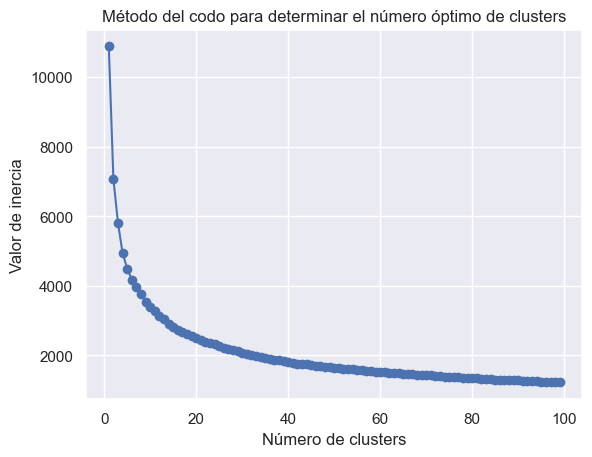
\includegraphics[width=0.4\textwidth]{charts/elbow_method_optimum_value.png}
    \caption{Elbow method}
    \label{fig:elbowmethod}
\end{figure}

Para la reducción de dimensionalidad, se utilizó el Análisis de Componentes Principales (PCA), que es una técnica para transformar un conjunto de datos de alta dimensión en uno de menor dimensión. Esto se logra proyectando los datos en un nuevo espacio formado por las direcciones (componentes principales) en las que los datos tienen la mayor variación. La reducción de dimensionalidad permite visualizar y analizar los datos de manera más eficiente y puede revelar patrones ocultos en los datos.

Después de aplicar el algoritmo de clustering y reducción de dimensionalidad, se obtuvieron las agrupaciones y se visualizaron en un gráfico de dispersión bidimensional.

\begin{figure}[h]
    \centering
    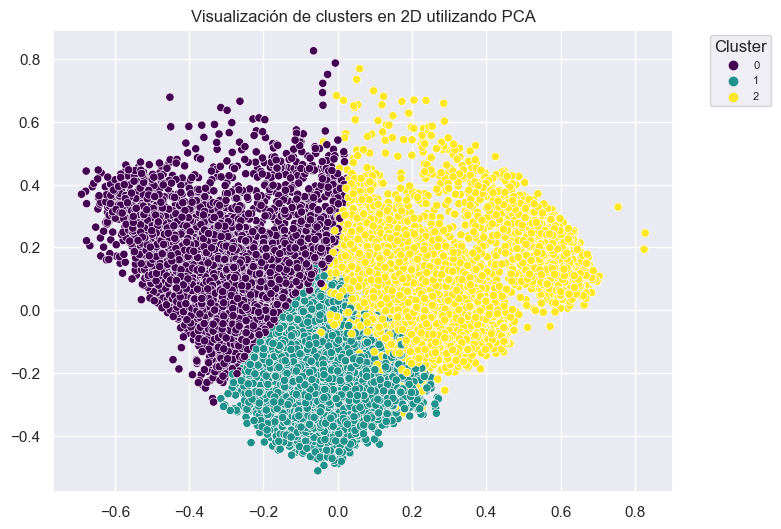
\includegraphics[width=0.4\textwidth]{charts/normalized/kmn_pca.png}
    \caption{Análisis de componentes principales}
    \label{fig:principalcomponentanalysis}
\end{figure}

En el caso de no aplicar la agrupación por dimensionalidad nos queda algo así:

\begin{figure}[h]
    \centering
    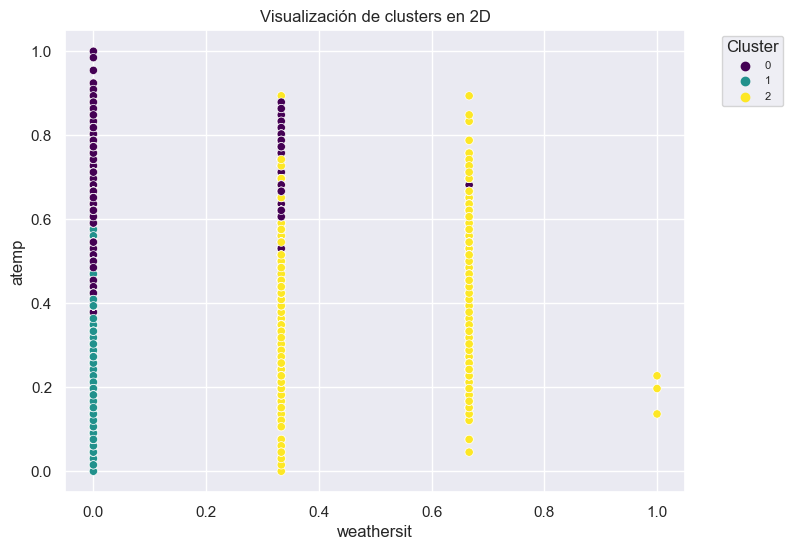
\includegraphics[width=0.4\textwidth]{charts/normalized/kmn_without_pca.png}
    \caption{Análisis de componentes principales sin agrupación}
    \label{fig:principalcomponentanalysiswithoutpca}
\end{figure}

Sin aplicar PCA, los datos se visualizan en su espacio de características original. Al representar los puntos en función de dos características específicas, se observa que los puntos se agrupan en filas o columnas, lo que dificulta la identificación de patrones o tendencias en los datos. Esto puede deberse a que las dos características elegidas no capturan la mayoría de la varianza en los datos, y las estructuras subyacentes están ocultas en otras dimensiones.
Al aplicar PCA a los datos, se transforman en un nuevo espacio de características, en el que los componentes principales capturan la mayor parte de la varianza en los datos. Al visualizar los datos en función de los primeras dos componentes principales, las estructuras subyacentes son más evidentes, ya que estos componentes representan la mayor parte de la información en los datos.

La matriz de confusión obtenida ha sido esta:
\begin{figure}[h]
    \centering
    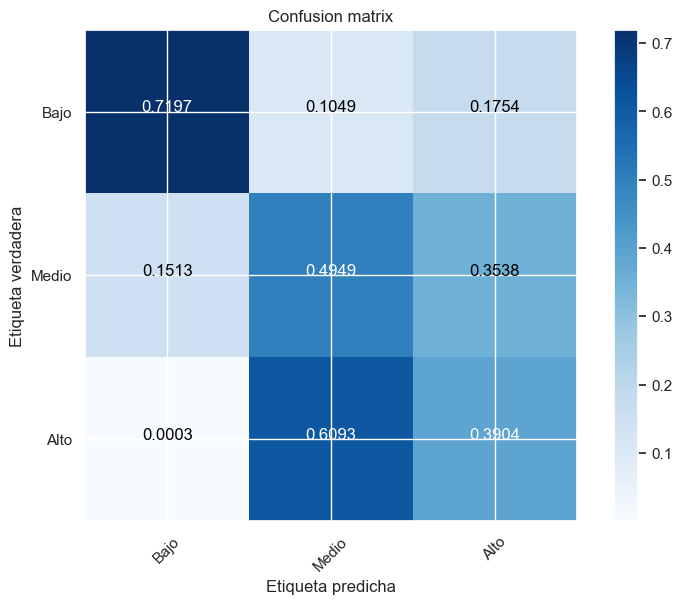
\includegraphics[width=0.4\textwidth]{charts/normalized/kmn_matrix_confussion.png}
    \caption{Matriz de confusión del aprendizaje no supervisado}
    \label{fig:kmnmatrizconfussion}
\end{figure}

\section{Evaluación del modelo de aprendizaje no supervisado}

En esta sección, evaluamos el modelo de aprendizaje no supervisado utilizando diversas métricas y discutimos su relevancia en el contexto del problema de predicción del número de bicicletas alquiladas en una hora determinada. A continuación, se presentan los valores de las métricas obtenidas y se explica su significado.

\subsection{Coeficiente de silueta promedio}

El coeficiente de silueta promedio es una medida de la calidad de los agrupamientos generados por un algoritmo de agrupamiento. Este coeficiente varía entre -1 y 1, donde un valor cercano a 1 indica que los grupos están bien separados y un valor cercano a -1 indica que los grupos están mal separados. En este caso, el coeficiente de silueta promedio obtenido es 0.2495.

\begin{itemize}
    \item \textbf{Valor obtenido:} 0.2495
\end{itemize}

\subsection{Inercia}

La inercia es una medida de la dispersión interna de los grupos y se calcula como la suma de las distancias al cuadrado de cada punto al centroide de su grupo. Un valor de inercia más bajo indica una mejor calidad de agrupamiento. En este caso, la inercia obtenida es 1841.0286.

\begin{itemize}
    \item \textbf{Valor obtenido:} 1841.0286
\end{itemize}

\subsection{Índice ARI}

El índice Adjusted Rand Index (ARI) es una medida de similitud entre dos agrupamientos, en este caso, el agrupamiento generado por el modelo y el agrupamiento real (etiquetas verdaderas). El ARI varía entre -1 y 1, donde un valor cercano a 1 indica que los dos agrupamientos son casi idénticos y un valor cercano a -1 indica que los agrupamientos son completamente diferentes. En este caso, el índice ARI obtenido es 0.2245.

\begin{itemize}
    \item \textbf{Valor obtenido:} 0.2245
\end{itemize}

\subsection{Índice AMI}

El índice Adjusted Mutual Information (AMI) es otra medida de similitud entre dos agrupamientos que tiene en cuenta la información mutua entre ellos, ajustada para tener en cuenta la posibilidad de obtener valores altos de información mutua por casualidad. El AMI varía entre 0 y 1, donde un valor cercano a 1 indica que los dos agrupamientos son casi idénticos y un valor cercano a 0 indica que no hay relación entre los agrupamientos. En este caso, el índice AMI obtenido es 0.2468.

\begin{itemize}
    \item \textbf{Valor obtenido:} 0.2468
\end{itemize}

\subsection{Matriz de confusión}
A partir de la matriz de confusión, podemos observar lo siguiente:
\begin{enumerate}
    \item El modelo es bastante preciso al predecir la clase ``Bajo'', con un 71.97\% de las predicciones correctas. Sin embargo, también hay una proporción significativa de casos clasificados incorrectamente como ``Medio'' (10.49\%) y ``Alto'' (17.54\%).
    \item En el caso de la clase ``Medio'', el modelo tiene una precisión del 49.49\%. Aproximadamente el 35.38\% de los casos en esta clase se clasificaron incorrectamente como ``Alto'' y el 15.13\% como ``Bajo''.
    \item Para la clase ``Alto'', el modelo tiene un rendimiento más bajo, con solo el 39.04\% de las predicciones correctas. El 60.93\% de los casos se clasificaron incorrectamente como ``Medio'', mientras que apenas el 0.03\% se clasificó como ``Bajo''.
\end{enumerate}
Estos resultados sugieren que el modelo de aprendizaje no supervisado tiene un rendimiento moderado en la predicción de la cantidad de bicicletas alquiladas en función de las características proporcionadas. El modelo tiene un rendimiento aceptable al predecir la clase ``Bajo'', pero su precisión es menor en las clases ``Medio'' y ``Alto''. Esto podría deberse a la dificultad de separar estas clases utilizando solo el algoritmo k-means y PCA.

\section{Discusión crítica}

En este estudio, se han explorado dos enfoques diferentes para predecir el número de bicicletas alquiladas en un momento específico del día: un modelo de \textbf{aprendizaje supervisado} y un modelo de \textbf{aprendizaje no supervisado}. A continuación, se presenta una comparación crítica de ambos enfoques en relación con nuestro objetivo y su posible utilización en el futuro.

\subsection{Aprendizaje supervisado}

El modelo de aprendizaje supervisado, basado en la \textbf{regresión lineal}, ha demostrado un excelente rendimiento en la predicción del número de bicicletas prestadas en función de diversas características. El \textbf{Error Cuadrático Medio (MSE)} es extremadamente bajo ($8.209062916187086e-22$), lo que sugiere que el modelo se ajusta muy bien a los datos. Además, el \textbf{Coeficiente de Determinación (R$^2$)} es 1.0, lo que indica un ajuste perfecto del modelo a los datos.

Dado su alto rendimiento, el modelo de aprendizaje supervisado sería útil para predecir con precisión el número de bicicletas alquiladas en momentos específicos del día y podría ser utilizado para tomar decisiones informadas sobre la gestión de recursos, la promoción de ofertas y la planificación de mejoras en la infraestructura de bicicletas compartidas.

\subsection{Aprendizaje no supervisado}

El modelo de aprendizaje no supervisado, basado en el algoritmo de \textbf{K-means}, ha demostrado un rendimiento moderado en la clasificación de las diferentes clases de alquileres de bicicletas (bajo, medio y alto). Aunque algunos indicadores, como el \textbf{Índice ARI} y el \textbf{Índice AMI}, sugieren que hay cierta similitud entre los agrupamientos generados por el modelo y las etiquetas verdaderas, hay margen de mejora en la precisión del agrupamiento.

El enfoque de aprendizaje no supervisado puede proporcionar información útil sobre la estructura subyacente de los datos y ayudar a identificar patrones y tendencias en el alquiler de bicicletas. Sin embargo, su rendimiento en la predicción del número exacto de bicicletas alquiladas en momentos específicos del día puede ser inferior al del modelo de aprendizaje supervisado.

\subsection{Limitaciones}

A pesar de los resultados prometedores obtenidos en este estudio, es importante reconocer algunas limitaciones que pueden afectar la generalización y aplicabilidad de los modelos en diferentes contextos y escenarios.

\subsubsection{Sobreajuste en el modelo supervisado}

Dado que el modelo de aprendizaje supervisado muestra un \textbf{ajuste perfecto} a los datos de entrenamiento, existe la posibilidad de que haya \textbf{sobreajuste} en el modelo. El sobreajuste se produce cuando el modelo se ajusta demasiado a los datos de entrenamiento y no generaliza bien a nuevos datos. Esto podría limitar la efectividad del modelo al enfrentarse a situaciones no vistas previamente o al aplicarse en diferentes ubicaciones y contextos.

\subsubsection{Calidad de las etiquetas en el modelo no supervisado}

La efectividad del modelo de aprendizaje no supervisado se basa en gran medida en la calidad de las \textbf{etiquetas} utilizadas para evaluar el agrupamiento. En este estudio, las etiquetas se han generado utilizando un enfoque basado en \textbf{cuartiles}, lo que podría no ser óptimo para capturar las diferencias reales en los patrones de alquiler de bicicletas. Una técnica de etiquetado diferente o más sofisticada podría mejorar la evaluación y el rendimiento del modelo no supervisado.

\subsubsection{Factores no considerados}

Tanto el modelo supervisado como el no supervisado se basan en un conjunto limitado de \textbf{variables} que se consideraron relevantes para el alquiler de bicicletas. Sin embargo, es posible que existan otros factores que influyan en el alquiler de bicicletas y que no se hayan tenido en cuenta en este estudio, como eventos especiales, cambios en las políticas de transporte o incluso la ubicación de las estaciones de alquiler.

\subsubsection{Limitaciones temporales}

Los modelos desarrollados en este estudio se basan en datos históricos hasta \textbf{septiembre de 2021}. Dado que los patrones de movilidad y los factores que influyen en el alquiler de bicicletas pueden cambiar con el tiempo, es crucial actualizar y validar los modelos regularmente utilizando datos más recientes para garantizar que sigan siendo precisos y relevantes.

\section{Conclusiones y Trabajo Futuro}

\subsection{Conclusiones}

En este estudio, se ha explorado el uso de modelos de aprendizaje supervisado y no supervisado para predecir el número de bicicletas alquiladas en función de diversas variables, como el clima, la temperatura, la velocidad del viento, la humedad y el tipo de usuario. El modelo de aprendizaje supervisado, basado en la regresión lineal, mostró un ajuste perfecto a los datos, aunque puede estar sujeto al sobreajuste. Por otro lado, el modelo de aprendizaje no supervisado, basado en el algoritmo k-means, proporcionó resultados moderados, pero con un margen de mejora.

Ambos enfoques han demostrado ser útiles para abordar el problema del alquiler de bicicletas. Sin embargo, se deben tener en cuenta las limitaciones identificadas en la sección de discusión crítica al aplicar estos modelos en diferentes contextos y al tomar decisiones basadas en sus resultados.

\subsection{Trabajo Futuro}

Dado que siempre hay margen de mejora en la predicción y el análisis de datos, se proponen las siguientes direcciones para el trabajo futuro:

\begin{itemize}
    \item \textbf{Mejorar el rendimiento del modelo supervisado}: Utilizar técnicas de regularización, como la regresión de Lasso o Ridge, para abordar el posible sobreajuste en el modelo supervisado y mejorar su capacidad de generalización.
    \item \textbf{Explorar otros algoritmos de aprendizaje no supervisado}: Probar diferentes algoritmos de agrupamiento, como DBSCAN o HDBSCAN, para mejorar la evaluación y el rendimiento del modelo no supervisado.
    \item \textbf{Incorporar más variables}: Investigar y agregar otras variables que puedan ser relevantes para el alquiler de bicicletas, como la ubicación de las estaciones de alquiler o datos sobre eventos especiales y políticas de transporte.
    \item \textbf{Actualizar y validar los modelos con datos más recientes}: A medida que estén disponibles nuevos datos, actualizar y validar los modelos para garantizar que sigan siendo precisos y relevantes en el tiempo.
    \item \textbf{Implementar modelos de aprendizaje profundo}: Explorar la aplicación de modelos de aprendizaje profundo, como redes neuronales, para mejorar la precisión de las predicciones y adaptarse a patrones más complejos en los datos.
    \item \textbf{Analizar el impacto de las intervenciones}: Investigar cómo diferentes intervenciones, como la promoción del uso de bicicletas o la mejora de la infraestructura, pueden afectar el alquiler de bicicletas y utilizar los modelos desarrollados para evaluar su efectividad.

\end{itemize}

Al seguir estas direcciones, este trabajo puede contribuir aún más al entendimiento y la predicción del alquiler de bicicletas, lo que a su vez puede ayudar a informar políticas y decisiones de transporte más efectivas y sostenibles.



\section*{Bibliografía}

\begin{thebibliography}{9}

    \bibitem{datasciencecentral}
    Brownlee, J. (2017).
    \textit{How to Prepare Data For Machine Learning}.
    Retrieved from Data Science Central: \url{https://machinelearningmastery.com/how-to-prepare-data-for-machine-learning/}

    \bibitem{machinelearningmastery}
    Brownlee, J. (2018).
    \textit{Introduction to Principal Component Analysis (PCA)}.
    Retrieved from Machine Learning Mastery: \url{https://machinelearningmastery.com/principal-components-analysis-for-dimensionality-reduction-in-python/}

    \bibitem{datasciencecentral}
    Brownlee, J. (2017).
    \textit{How to Prepare Data For Machine Learning}.
    Retrieved from Data Science Central: \url{https://www.datasciencecentral.com/profiles/blogs/how-to-prepare-data-for-machine-learning}

    \bibitem{barcelonageeks}
    Barcelona Geeks. (2022).
    \textit{Método del codo para el valor óptimo de k en k-means}.
    Retrieved from Barcelona Geeks: \url{https://barcelonageeks.com/metodo-del-codo-para-el-valor-optimo-de-k-en-kmeans/}

    \bibitem{scikit-learn}
    Scikit-learn. (2022).
    \textit{Adjusted Rand Index}.
    Retrieved from Scikit-learn: \url{https://scikit-learn.org/stable/auto_examples/cluster/plot_adjusted_for_chance_measures.html}

    \bibitem{aprendemachinelearning}
    Aprende Machine Learning. (2022).
    \textit{k-means en Python paso a paso}.
    Retrieved from Aprende Machine Learning: \url{https://www.aprendemachinelearning.com/k-means-en-python-paso-a-paso/}

    \bibitem{datasourceai}
    Datasource.ai. (2022).
    \textit{Comprensión de la matriz de confusión y cómo implementarla en Python}.
    Retrieved from Datasource.ai: \url{https://www.datasource.ai/es/data-science-articles/comprension-de-la-matriz-de-confusion-y-como-implementarla-en-python}

    \bibitem{cienciadedatos}
    Ciencia de Datos. (2022).
    \textit{Regresión lineal en Python}.
    Retrieved from Ciencia de Datos: \url{https://www.cienciadedatos.net/documentos/py10-regresion-lineal-python.html}

    \bibitem{codigopiton}
    Código Piton. (2022).
    \textit{Cómo hacer un histograma en Python}.
    Retrieved from Código Piton: \url{https://www.codigopiton.com/como-hacer-un-histograma-en-python/#:~:text=Para%20hacer%20un%20histograma%20en%20Python%20es%20necesario,librer%C3%ADa%20como%20Matplotlib%2C%20Seaborn%2C%20Bokeh%2C%20Altair%20o%20Plotly.}

\end{thebibliography}


% \appendices
% \section{}
% Appendix uno va aquí.

% % you can choose not to have a title for an appendix
% % if you want by leaving the argument blank
% \section{}
% Appendix dos va aquí.


% use section* for acknowledgment
\bibliographystyle{IEEEtran}
%% you can change the style into any other styles available, I personally love IEEEtran.
\bibliography{citations}
%% to generate references, input the name of your .bib file and cite anywhere in the document.

\end{document}
